\chapter{Literature Review}% Main chapter title
\thispagestyle{nohead}
\label{LitReview} % For referencing the chapter elsewhere, use \ref{LitReview} 

%----------------------------------------------------------------------------------------

\where incorporates ideas from at least three separate disciplines: software verification, machine learning, and software measurement and metrics. Each of these disciplines has a considerable body of research associated with it. This chapter focusses on the intersections of the three areas while addressing to relevant literature from each individual area.
A Venn diagram illustrating how the literature was classified is given in Figure \ref{fig:litreview}. 
%It can be seen that the intersection of \textit{software verification} and \textit{measurement/metrics} itself contains two separate categories of interest: benchmarks and competitions in formal methods, and the relatively young field of \textit{proof engineering}.
The rest of this chapter will review the literature associated with each segment of Figure \ref{fig:litreview} - moving clockwise from the software verification circle.


\begin{figure}

\centering
\def\firstcircle{(3cm,0cm) circle (2.5cm)}
\def\secondcircle{(0cm,0cm) circle (2.5cm)}
\def\thirdcircle{(1.5cm,3cm) circle (2.5cm)}
% Suppose we have three circles or ellipses or whatever. Let us define
% commands for their paths since we will need them repeatedly in the
% following:
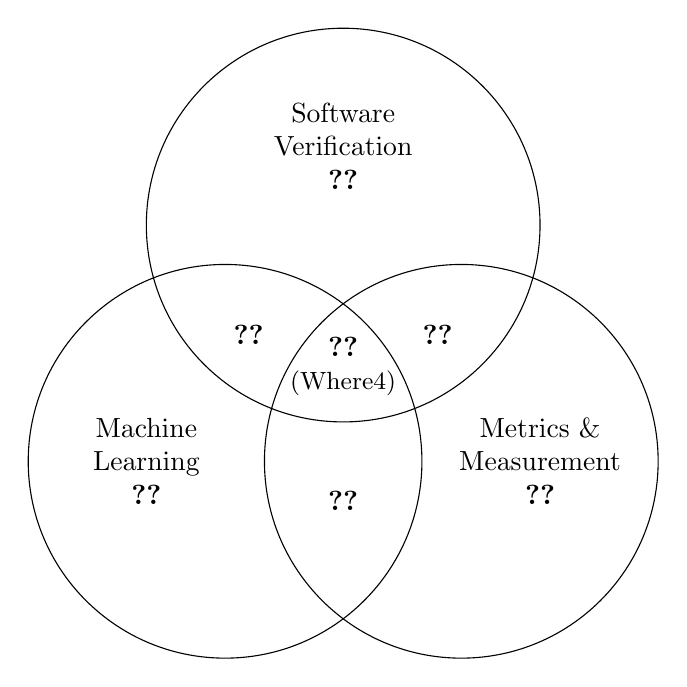
\begin{tikzpicture}
	
	\draw \firstcircle node [below] {};
	\draw \secondcircle node [above] {};
	\draw \thirdcircle node [below] {};
	\node[align=center] at (-1cm, 0cm) {Machine\\Learning\\ \ref{sec:lrml} };
	\node[align=center] at (1.5cm, 4cm) {Software\\Verification\\ \ref{sec:lrsv}};
	\node[align=center] at (4cm, 0cm) {Metrics \&\\ Measurement\\ \ref{sec:lrmm}};
	\node[align=center] at (1.5cm, 1.2cm) {\ref{sub:lrsvmmml}\\\small{(Where4)} };
	\node[align=center] at (0.3cm, 1.6cm) {\ref{sub:lrsvml}};
	\node[align=center] at (2.7cm, 1.6cm) {\ref{sub:lrsvmm}};
	\node[align=center] at (1.5cm, -0.5cm) {\ref{sub:lrmmml}};
	
\end{tikzpicture}

\caption{\where as placed at the intersection of three disciplines}
\label{fig:litreview}

\end{figure}


\section{Software Verification Systems}
\label{sec:lrsv}

An overview of the \why verification system \cite{why:shephard,why:whereprovers} has been given in the previous chapter. The WhyML programming language provides a high-level ML-like language for the specification of programs with pre- and post- conditions, recursive definitions and type invariants. An extensive library of verified polymorphic data-types make WhyML a flexible language \cite{verifythis,why:polymorphic}. As we stated in the previous chapter, it is \why's driver-based approach to interfacing with external tools that is of most interest to our project. This approach is in contrast to the typical SV system of tightly-integrated systems consisting of an IDE/annotation language/front-end DSL, intermediate logic language, and SMT-solving back-end. Examples of systems which follow this model are Spec\# \cite{spec} and Dafny \cite{Dafny} which use the Boogie \cite{Boogie} intermediate language and the Z3 \cite{Z3} SMT solver.

The diversity of languages and formalisms has been matched by an increase in software \textit{tools} in recent years. Filli{\^a}tre's overview of the deductive verification tool landscape \cite{deductiveSV} counts 65 tools cited or used in the five papers of a special edition of the \textit{Verified Software: Theory, Tools and Experiments} workshop. There has been an effort to make these tools more interoperable. The two-dozen ATPs, ITPs and SMT solvers targeted by \why makes it an attractive choice for translations: recent projects have used \why as a platform for discharging POs translated from Boogie \cite{b2w} and the B system \cite{rodinplugin,atelierB2w}. 

\subsection{Measurement and Metrics in Software Verification}
\label{sub:lrsvmm}

With the diversity of approaches currently in use in the SV domain, experimental software measurement concepts and techniques must be introduced for the rigorous evaluation, comparison, and characterisation of software. These techniques are usually employed in the general software engineering domain and have been adapted for the specific concerns of formal methods. 

The intersection of SV and empirical SE disciplines can be further broken into the three subsections to follow.      

\subsubsection{Software Verification Competitions}
\label{sub:lrsvmmbench}

At present, competitions provide the most prominent means of comparing systems which focus on the verification of object-oriented software. In competitions such as those held at FoVeOOS 2011 \cite{bormer:hal-00789525} and the VerifyThis series \cite{Huisman2015}, teams are given the natural-language specifications for a small number of typical SV problems. Any system can be used, with tool developers often choosing to use their own system. Many of the \why gallery of verified programs originated from software verification competitions \cite{verifythis} 

The situation for automatic program verifiers which use model-checking techniques to ensure properties (such as reachability or termination) is similar: a well-established competition, SV-COMP \cite{SVCOMP}, is held annually. Importantly, a large benchmark repository consisting of competition questions is available. This is made possible due to the standard input format of the tools: all accept input in the C language. Other efforts to standardise benchmark repositories for software verification tools are discussed in the next subsection.  

\subsubsection{Benchmark Repositories}

The need for a standard set of benchmarks for the diverse range of verification systems was identified by a number of participants in the week-long seminar at Dagstuhl \cite{Dagstuhl} in 2014. The series of workshops and events brought the model-checking and SV system communities together. Qualitative, repeatable comparative evaluation was agreed as an important goal for formal methods to advance as a software engineering discipline. The VACID-0 \cite{Leino10vacid-0:verification} project is an attempt to maintain a repository of standard abstract specifications for deductive software verification tasks similar to those used in the VerifyThis competition.  

The benefits of such a benchmark suite are identified by the SMT-LIB \cite{SMTLIB} project. The performance of SMT solvers has significantly improved in recent years due in part to the standardisation of an input language and the use of standard benchmark programs in competitions \cite{SMTEVAL2013}. \why uses the SMT-LIB language as input format for a number of SMT solvers (including CVC4, Z3, and veriT). Our previous work \cite{Healy:2016} has exploited this feature to characterise verification tasks  compared to other application domains of SMT solvers.

The TPTP (Thousands of Problems for Theorem Provers) project \cite{TPTP} is a benchmark repository with similar aims but a wider scope. The problems target theorem provers which specialise in numerical problems as well as general-purpose SAT and SMT solvers. The TPTP library is specifically designed for the rigorous experimental comparison of solvers \cite{Sutcliffe200139}. There has been significant development effort by \why developers to support the TPTP format in \why and to extend the TPTP language with rank-1 polymorphism \cite{why:tptp}. 

\subsubsection{Proof Engineering}
\label{sub:lrsvmmpe}

The scale of formal software engineering projects has grown in recent years. The formal verification of the seL4 microkernel \cite{Klein:2014:CFV} and Thomas Hales' \textit{FlySpeck} proof of the Kepler Conjecture \cite{hales-kepler} were large and complicated engineering projects developed over a number of years. Both projects represent significant engineering efforts and produced a large volume of software artefacts in the form of \textit{proof scripts}. Researchers applying concepts from software engineering to mangae and measure such projects call their practice ``proof engineering'' \cite{Klein2014}.

Aspinall and Kaliszyk \cite{Aspinall2016} suggest adapting the standard Chidamber and Kemerer \cite{CandK} (``C\&K'') metrics commonly used tor measure object-oriented software (OOS). Both OOS and formal proofs make use of ``modules'' to package related classes and lemmas/axioms respectively. The authors use this analogy to model  and measure the dependency tree for proof modules, the module's  coupling and cohesion metrics. These metrics will be discussed further in Section \ref{sec:lrmm}.

Other approaches measure syntactic features of the specification to derive complexity metrics. The \textit{size} of a formal proof script was found to be quadratically related to the human effort (and associated cost) of large-scale formal engineering projects \cite{CostIndicator}. 
The verification of the seL4 microkernel mentioned previously was used as the basis for this study.
       

\section{Software Measurement and Metrics}
\label{sec:lrmm}
%also include the experimental process
%cite the metrics book

\subsection{Measurement and Machine Learning}
\label{sub:lrmmml}
%mention two journals: Empirical Software Enginnering, one that James said

\section{Machine Learning}
\label{sec:lrml}

\subsection{Verification and Machine Learning}
\label{sub:lrsvml}

\subsection{Where4 and the intersection of all three disciplines}
\label{sub:lrsvmmml}

\section{Conclusion}
